\documentclass[border=10pt]{standalone}
\usepackage[european]{circuitikz}
\begin{document}
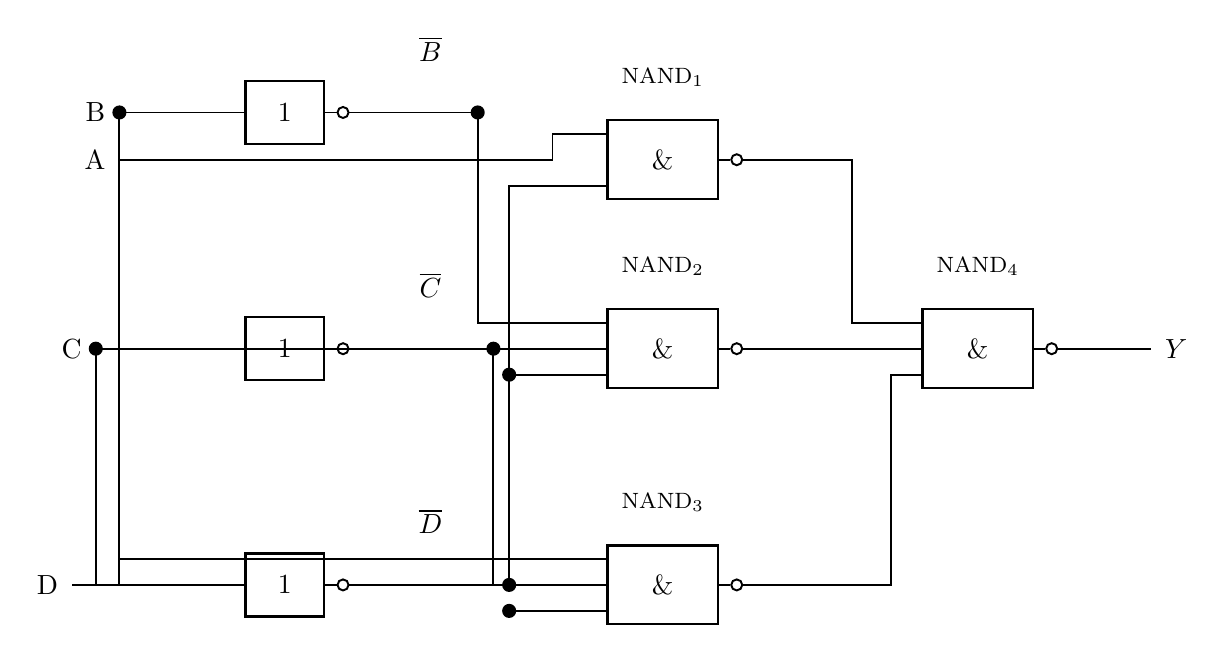
\begin{tikzpicture}[line width=0.7pt, font=\normalsize,
  dot/.style={circle, fill, inner sep=1.8pt}]

% 习题 7.14 两级与非：Y = NAND(p1,p2,p3)
%   p1 = NAND2(A, D̄)        —— 2 输入
%   p2 = NAND3(B̄, C, D̄)   —— 3 输入
%   p3 = NAND3(B, C̄, D̄)   —— 3 输入
% 087 打回项全部处理：输入数可读、T 形实心点、纯交叉无点、标签离走线、门名离框。
% 坐标：源轨 x=-1.6；非门列 x=0..1.0；一级 NAND x=4.6..6.0；末级 x=8.6..10.0。
% 行 y：NAND1=9.0  NAND2=6.6  NAND3=3.6  非门 B=9.6 C=6.6 D=3.6  A 轨=9.0。

\newcommand{\notgate}[3]{% #1 y中心  #2 输入名  #3 输出名（框 x=0..1.0，出线到 2.6）
  \begin{scope}[shift={(0,#1-0.4)}]
    \draw[thick] (0,0) rectangle (1.0,0.8);
    \node at (0.5,0.4) {1};
    \draw (1.0,0.4) -- (1.16,0.4);
    \draw (1.24,0.4) circle (0.07);
    \draw (1.31,0.4) -- (2.6,0.4);
    \draw (0,0.4) -- (-0.7,0.4);
    \node[anchor=south] at (2.35,0.92) {#3};
  \end{scope}}
\newcommand{\nandgate}[4]{% #1 x #2 y中心 #3 名 #4 输入数
  \begin{scope}[shift={(#1,#2-0.5)}]
    \draw[thick] (0,0) rectangle (1.4,1.0);
    \node at (0.7,0.5) {\&};
    \node[anchor=south, font=\footnotesize] at (0.7,1.30) {#3};
    \draw (1.4,0.5) -- (1.56,0.5);
    \draw (1.64,0.5) circle (0.07);
    \draw (1.71,0.5) -- (2.3,0.5);
  \end{scope}}

% ── 原变量源轨（x=-1.6）：A 9.0 / B 9.6 / C 6.6 / D 3.6 ──
% 四条源轨各是一条竖线，从端子名右侧起向下到最低所需行
\draw (-1.6,9.0) -- (-1.6,9.0);   % A 端子（单点）
\node[anchor=east] at (-1.65,9.0) {A};
\draw (-1.6,9.6) -- (-1.6,3.6);   % B 轨（供 B 非门 + B 原变量）
\node[anchor=east] at (-1.65,9.6) {B};
\draw (-1.9,6.6) -- (-1.9,3.6);   % C 轨（供 C 非门 + C 原变量）
\node[anchor=east] at (-1.95,6.6) {C};
\draw (-2.2,3.6) -- (-2.2,3.6);   % D 端子（单点）
\node[anchor=east] at (-2.25,3.6) {D};
% 非门输入（从各自原变量轨水平进框）
\draw (-1.6,9.6) -- (-0.7,9.6);   % B → 非门
\draw (-1.9,6.6) -- (-0.7,6.6);   % C → 非门
\draw (-2.2,3.6) -- (-0.7,3.6);   % D → 非门
% 非门列
\notgate{9.6}{B}{$\overline{B}$}
\notgate{6.6}{C}{$\overline{C}$}
\notgate{3.6}{D}{$\overline{D}$}

% ── 源轨到 NAND 输入（每条线一个源，不共用干线；T 点只在分叉处）──
% A 原变量：y9.0 右行到 NAND1 上输入 9.33
\draw (-1.6,9.0) -- (3.9,9.0) -- (3.9,9.33) -- (4.6,9.33);
% B 原变量：B 轨 (-1.6,9.6) 下行到 3.93（NAND3 上输入）
\draw (-1.6,9.6) -- (-1.6,3.93) -- (4.6,3.93);
\node[dot] at (-1.6,9.6) {};      % B 轨起点 T（分出 B 非门 + B 原变量）
% C 原变量：C 轨 (-1.9,6.6) 下行到 6.60（NAND2 中输入）
\draw (-1.9,6.6) -- (-1.9,6.60) -- (4.6,6.60);
\node[dot] at (-1.9,6.6) {};
% B̄：非门出 (2.6,9.6) 下行到 6.93（NAND2 上输入）
\draw (2.6,9.6) -- (2.95,9.6) -- (2.95,6.93) -- (4.6,6.93);
\node[dot] at (2.95,9.6) {};
% C̄：非门出 (2.6,6.6) 下行到 3.60（NAND3 中输入）
\draw (2.6,6.6) -- (3.15,6.6) -- (3.15,3.60) -- (4.6,3.60);
\node[dot] at (3.15,6.6) {};
% D̄：非门出 (2.6,3.6) 上行到 8.67（NAND1 下输入），并在 6.27 / 3.27 分叉
\draw (2.6,3.6) -- (3.35,3.6) -- (3.35,8.67) -- (4.6,8.67);
\node[dot] at (3.35,3.6) {};
\draw (3.35,6.27) -- (4.6,6.27);   % → NAND2 下输入
\node[dot] at (3.35,6.27) {};
\draw (3.35,3.27) -- (4.6,3.27);   % → NAND3 下输入
\node[dot] at (3.35,3.27) {};

% ── 一级 NAND（2 / 3 / 3 输入，引脚等距可读）──
\nandgate{4.6}{9.0}{NAND$_1$}{2}   % 入 9.33(A) 8.67(D̄)
\nandgate{4.6}{6.6}{NAND$_2$}{3}   % 入 6.93(B̄) 6.60(C) 6.27(D̄)
\nandgate{4.6}{3.6}{NAND$_3$}{3}   % 入 3.93(B) 3.60(C̄) 3.27(D̄)

% ── 末级 NAND4：入 6.93(p1) 6.60(p2) 6.27(p3) ──
\nandgate{8.6}{6.6}{NAND$_4$}{3}
% p1 出 (6.9,9.0) → 下折 6.93
\draw (6.9,9.0) -- (7.7,9.0) -- (7.7,6.93) -- (8.6,6.93);
% p2 出 (6.9,6.6) → 直入 6.60
\draw (6.9,6.6) -- (8.6,6.6);
% p3 出 (6.9,3.6) → 上折 6.27
\draw (6.9,3.6) -- (8.2,3.6) -- (8.2,6.27) -- (8.6,6.27);
% Y
\draw (10.9,6.6) -- (11.5,6.6);
\node[anchor=west] at (11.55,6.6) {$Y$};

\end{tikzpicture}
\end{document}
